% This LaTeX was auto-generated from MATLAB code.
% To make changes, update the MATLAB code and export to LaTeX again.

\documentclass{article}

\usepackage[utf8]{inputenc}
\usepackage[T1]{fontenc}
\usepackage{lmodern}
\usepackage{graphicx}
\usepackage{color}
\usepackage{hyperref}
\usepackage{amsmath}
\usepackage{amsfonts}
\usepackage{epstopdf}
\usepackage[table]{xcolor}
\usepackage{matlab}

\sloppy
\epstopdfsetup{outdir=./}
\graphicspath{ {./lab1_images/} }

\begin{document}

\begin{matlabcode}
% inputting calibration data
voltage_cali = [212; 232; 300; 370; 432; 505; 573; 630; 680; 737; 769];
angle_cali = [-90; -80; -60; -40; -20; 0; 20; 40; 60; 80; 90];

% creating a trendline
p = polyfit(voltage_cali, angle_cali, 1);
px = [min(voltage_cali) max(voltage_cali)];
py = polyval(p, px);

clf
scatter(voltage_cali, angle_cali, "filled")
hold on
plot(px, py, 'LineWidth', 2);
title("Angle vs Voltage")
xlabel("Voltage (mV)")
ylabel("Angle (°)")
legend('Calibration points', sprintf('y=%f*x+%f',p(1), p(2)));
hold off
\end{matlabcode}
\begin{center}
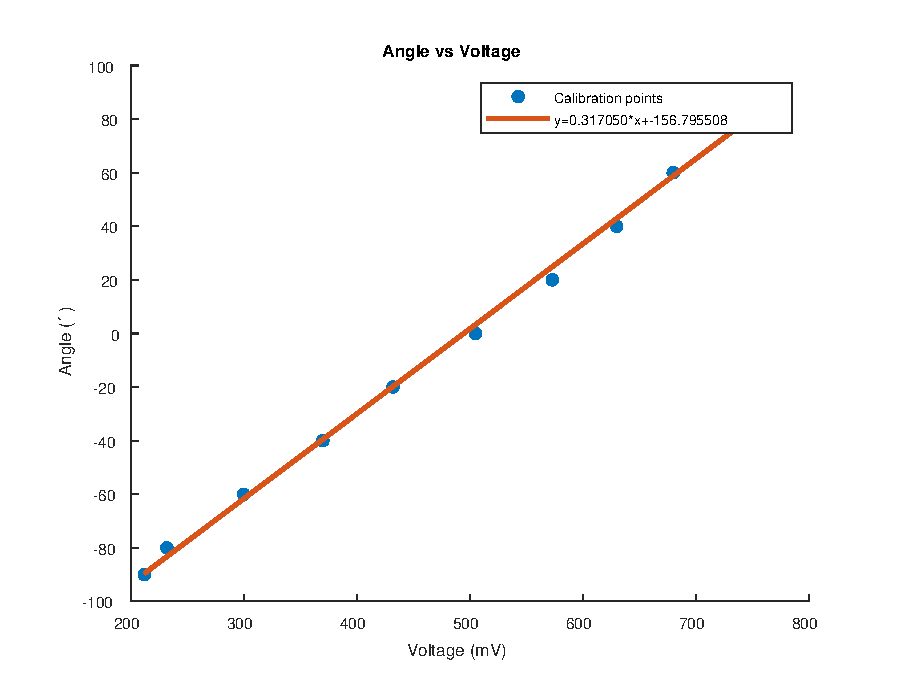
\includegraphics[width=\maxwidth{56.196688409433015em}]{figure_0.eps}
\end{center}
\begin{matlabcode}


% calculating the angle data from the trendline
exp_data = readmatrix('pendulum_voltage.csv');
voltage_exp = exp_data(:,2) * 1000; % convert from V to mV
time_exp = exp_data(:,1) + 15;

angle_exp = polyval(p, voltage_exp);

plot(time_exp, angle_exp); hold on
axis([0 30 -90 90])
title("Angle vs Time")
xlabel("Time (sec)")
ylabel("Angle (°)"); hold off
\end{matlabcode}
\begin{center}
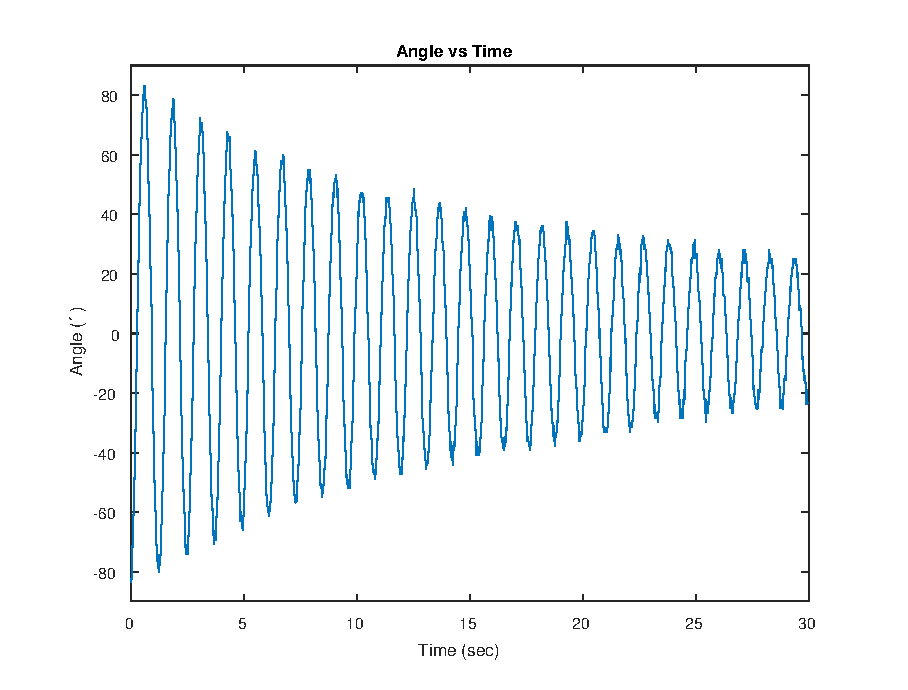
\includegraphics[width=\maxwidth{56.196688409433015em}]{figure_1.eps}
\end{center}
\begin{matlabcode}


\end{matlabcode}

\end{document}
